\begin{center}
\section{Research: Look-Ahead Heuristic}
\end{center}

Look-ahead(LA) has many different definitions\cite{HARALICK1980263}, but for a deterministic system, knowledge of future outcomes(states) can be determined if the current state is known; this is defined as foresight, and it can be used to evaluate options more intelligently\cite{sharma2024notelookaheadreallife}.

As mentioned in Section\ref{Look-ahead}, look-ahead algorithms and their design have already been adopted to solve the Travelling Salesman Problem and its variants. In Section\ref{NN-Look-ahead}, the greedy Nearest Neighbour Search algorithm was employed for the STSP to conform to the look-ahead algorithm proposed in their research. This is not possible for the Cheapest Insertion Heuristic.

\subsection{Problem To Solve}
\label{problem}
Greedy heuristics rarely produce global optimal solutions because they only evaluate locally optimal decisions, whereas the exact solution makes trade-offs at the local level to achieve better gains globally\cite{BANGJENSEN2004121}. These pitfalls are often hard to spot and are practically irreversible once made, especially in TSP\cite{GUTIN200281}.

% \begin{figure}[!ht]
%     \centering
%     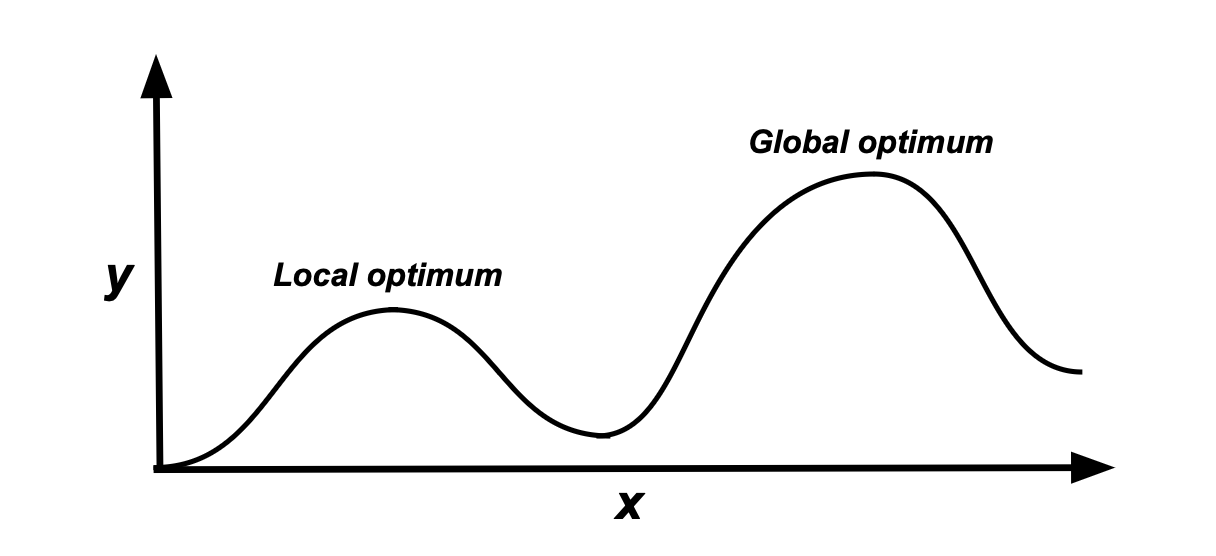
\includegraphics[width=\textwidth]{sections/image/Hill_climb.png}
%     \caption{Local Optimal vs Global Optimal Illustration}
%     \cite{hill_climbing_medium}
% \end{figure}

The cause of local optimal pitfalls varies for each algorithm, but for the CIH(Section\ref{CIH}), the pitfall occurs when a cluster is chosen because a single node is closest to the route, whereas a better cluster construction is possible in another way.

\begin{figure}[H]
    \centering
    \begin{minipage}{0.33\textwidth}
        \centering
        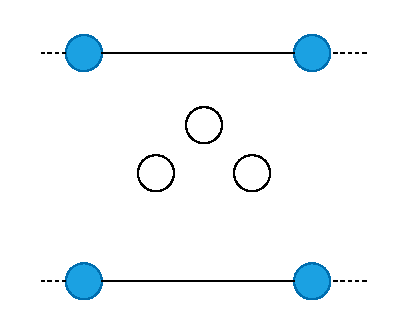
\includegraphics[page=1, width=1.2\textwidth]{sections/image/dissertationdemo.drawio.pdf}
        \caption{Base Problem}
        \label{fig:tsp_problem}
    \end{minipage}\hfill
    \begin{minipage}{0.33\textwidth}
        \centering
        \includegraphics[page=2, width=1.2\textwidth]{sections/image/dissertationdemo.drawio.pdf}
        \caption{Incorrect Solution}
        \label{fig:CIH_solution}
    \end{minipage}\hfill
    \begin{minipage}{0.33\textwidth}
        \centering
        \includegraphics[page=3, width=1.2\textwidth]{sections/image/dissertationdemo.drawio.pdf}
        \caption{Correct Solution}
        \label{fig:TSP_Optimal}
    \end{minipage}
\end{figure}


In Figure\ref{fig:tsp_problem}, the base problem involves a partial route that passes through the top and bottom of a cluster of three nodes in the centre. CIH will construct the local optimal route(Figure\ref{fig:CIH_solution}) to the cluster in the order shown in the diagram based on picking local optimal options using the cost function(Equation\ref{CIH_Cost}). This is because the topmost node is closest to the route and therefore has the lowest cost, whereas picking one of the other suboptimal nodes would result in the global optimal solution(Figure\ref{fig:TSP_Optimal}).

\subsection{Static Look-Ahead Cheapest Insertion Heuristic(SLACIH)}
\label{SLACIH}
This report explains how a look-ahead search of static depth is applied to CIH. To help avoid pitfalls, a look-ahead design can be employed to guide decision-making\cite{DongLookahead}. Applying look-ahead to the Cheapest Insertion Heuristic(CIH) cannot be done in the same manner as the Look-Ahead Nearest Neighbour\cite {SARKAR19941}(Section\ref{NN-Look-ahead}); this is due to the nearest neighbour using a sequential head as a point of insertion, while CIH evaluates every node to be added anywhere in the route.

This report examines a new algorithm, the Static Look-Ahead Cheapest Insertion Heuristic(SLACIH), or look-ahead insertion for short. If a specific look-ahead depth is specified, it can be listed in brackets after the name, e.g. SLACIH(3) for a depth of 3. 

Designing an effective and working look-ahead algorithm requires the heuristic to create a wide variation in branching solutions, enabling efficient foresight to be achieved. Taking the intuitive approach of doing sequential CIH iterations will not be effective. This is because the probability of finding unique and relevant solutions is low, given that the CIH iterations are unrelated to past insertions. To solve this, a temporary path which contains only past insertions is used exclusively as the search space for evaluating CIH in the look-ahead. This divides the SLACIH search into two subprocesses:

\begin{itemize}
    \item Normal CIH search to find where it would be added to the partial path
    \item Temporary look-ahead search to find which nodes would be added next based on previous insertions
\end{itemize}

This preserves the properties of the CIH cost function(Equation\ref{CIH_Cost}), allowing nodes to be added anywhere in the route, provided that the look-ahead only considers options that are relevant. The steps of SLACIH are as follows:

\begin{legal}
    \item Generate an initial starting partial set \label{LAI_Init}
    \item For each unvisited node:  \label{LAI_For1}
    \begin{legal}
            \item Calculate the cost function of adding the node to every position in the partial route \label{LAI_CIH}
            \item Add the unvisited node and the two visited nodes found in 2.1 to a temporary route \label{LAI_CIH2}
            \item Set a new depth limit if the depth exceeds the number of unvisited nodes \label{LAI_CIH3}
            \item For each unvisited node:\label{LAI_For2}
            \begin{legal}
                \item Calculate the cost function of adding the node to every position in the temporary route\label{LAI}
                \item Add the cheapest node to the temporary\label{LAI2}
                \item Increases depth count by one \label{LAI3}
                \item Repeat step 2.4 until the desired look-ahead depth \label{LAI4}
            \end{legal}
    \end{legal}
    \item Calculate the temporary route length and compare against best known \label{LAI_Calc}
    \item Add the original node to the position found in step 2 \label{LAI_ADD}
    \item Repeat step 2 until there are no unvisited nodes \label{LAI_While}
\end{legal}

When comparing it to CIH, steps 1, 2.1, 4, and 5 are identical to those in CIH, with steps 2.2 to 3 forming part of the look-ahead design. The look-ahead design considers every node, $n$, against a partial route of size $depth+2$, for $depth$ iterations. Counting the nested For loops, the time complexity can be calculated:

\begin{equation}
O(\tcboxmath[boxmath={blue}{CIH}]{n^2 \cdot (n}+\tcboxmath[boxmath={red}{LA}]{n\cdot (\text{depth}+2)\cdot \text{depth}}))
\label{equ:statictime}
\end{equation}

\begin{tikzpicture}[remember picture, overlay, font=\sffamily]
\draw[blue,->] (CIH.north) --++(120:5mm) node[anchor=south]{CIH};
\draw[red,->] (LA.north) --++(70:5mm) node[anchor=south]{Look-ahead};
\draw[decorate, decoration={brace, mirror, raise=3pt, amplitude=2mm}] (CIH.south west)--(LA.south east) node[below=3mm, midway]{SLACHI Time Complexity};
\end{tikzpicture}

But can be simplified to $O(n^5)$:
\begin{gather*}
\begin{aligned}
    O(n^2 \cdot (n+n\cdot (\text{depth}+2) \cdot \text{depth})) & \quad \text{// Base equation} \\ 
    O(n^2 \cdot (n+n\cdot \text{depth}^2)) & \quad \text{// Simplify and ignore +2} \\ 
    O(n^3 + n^3\cdot \text{depth}^2) & \quad \text{// Expand brackets} \\ 
    O(n^3 + n^3\cdot n^2) & \quad \text{// Worse-case value of depth} \\
    O(n^3 +n^5) & \quad \text{// Simplify} \\ 
    O(n^5) & \quad \text{// Ignore lower-order terms}
\end{aligned}
\end{gather*}
Look-ahead depth can have values $n\geq\text{depth}\geq0$, allowing it to be applied to $n$ in Big O notation. It also shows that the time complexity is bound to a quintic polynomial(5th power), regardless of the depth of the look-ahead.

Visually, the logic of evaluating temporary routes can be illustrated in geometric cases for each iteration. Blue nodes represent visited nodes, white nodes represent unvisited nodes, the orange node represents the node being considered, and yellow lines and nodes represent the temporary route.

\begin{center}
    \textbf{Inner Working}
\end{center}

\begin{figure}[!ht]
    \centering
    \begin{minipage}{0.33\textwidth}
        \centering
        \includegraphics[page=8, width=1.2\textwidth]{sections/image/dissertationdemo.drawio.pdf}
        \caption{Node 1}
        \label{node1}
    \end{minipage}\hfill
    \begin{minipage}{0.33\textwidth}
        \centering
        \includegraphics[page=9, width=1.2\textwidth]{sections/image/dissertationdemo.drawio.pdf}
        \caption{Node 2}
    \end{minipage}\hfill
    \begin{minipage}{0.33\textwidth}
        \centering
       \includegraphics[page=10, width=1.2\textwidth]{sections/image/dissertationdemo.drawio.pdf}
        \caption{Node 3}
        \label{Node3}
    \end{minipage}
\end{figure}

Figures\ref{node1}-\ref{Node3} show SLACIH(1) with a look-ahead depth of one, evaluating each unvisited node with foresight in yellow. Unlike CIH(Figure\ref{fig:CIH_solution}), which incorrectly considers the northernmost node due to its close proximity to the route, SLACIH calculates the cost of adding the node and the next.


\begin{center}
    \textbf{Outer Working}
\end{center}

\begin{figure}[H]
    \centering
    \begin{minipage}{0.33\textwidth}
        \centering
        \includegraphics[page=4, width=1.2\textwidth]{sections/image/dissertationdemo.drawio.pdf}
        \caption{Iteration 1}
        \label{Itt1}
    \end{minipage}
    \begin{minipage}{0.33\textwidth}
        \centering
        \includegraphics[page=5, width=1.2\textwidth]{sections/image/dissertationdemo.drawio.pdf}
        \caption{Iteration 2}
    \end{minipage}
\end{figure}
\begin{figure}[!ht]
    \centering
    \begin{minipage}{0.33\textwidth}
        \centering
        \includegraphics[page=6, width=1.2\textwidth]{sections/image/dissertationdemo.drawio.pdf}
        \caption{Iteration 3}
        \label{Itt3}
    \end{minipage}
    \begin{minipage}{0.33\textwidth}
        \centering
        \includegraphics[page=7, width=1.2\textwidth]{sections/image/dissertationdemo.drawio.pdf}
        \caption{Solution}
        \label{Itt4}
    \end{minipage}
\end{figure}

Figures\ref{Itt1}-\ref{Itt4} show SLACIH(1) with a look-ahead depth of one, iteratively adding the next node to the route based on its evaluation of the cheapest temporary route found during the inner workings. In Figure\ref{Itt3}, there is no look-ahead(yellow lines) because there are no more unvisited nodes to visit. Therefore, the look-ahead depth is defined by:

\begin{equation}
    \text{depth} = \min(\text{depth}, \text{\# of unvisited nodes}) = \min(\text{depth}, |\text{graph}|-|\text{route}|-1)
\end{equation}


\pagebreak
\subsubsection{Pseudocode}

\begin{algorithm}[H]
\caption{SLACIH$(depth : \text{integer}, g: \text{Graph})$}
\begin{algorithmic}[1]
\State $path := \text{initial partial set}$ \Comment{Random node or Convex Hull(Step\ref{LAI_Init})}
\While{$\exists$ node $\notin$ path} \Comment{Step\ref{LAI_While}}
    \State $[b\_node,\ b\_position,\ b\_cost] := \text{default values}$
    \For{node $\notin$ path} \Comment{Step\ref{LAI_For1}}
        \State [node, position, cost] = CIH-Search$(depth,\ node,\ path, g)$
        \If{$cost < b\_cost$} \Comment{Step\ref{LAI_Calc}}
            \State $[b\_node,\ b\_position,\ b\_cost] = [node,\ position,\ cost]$
        \EndIf
    \EndFor
    \State path.add(b\_node, b\_position)\Comment{Step\ref{LAI_ADD}}
\EndWhile
\end{algorithmic}
\end{algorithm}

\begin{algorithm}[H]
\caption{CIH-Search$(\text{depth} : \text{integer}, n : \text{Node}, \text{path} : \text{route},g : \text{graph})$}
\begin{algorithmic}[1]
\State $[b\_position,\ b\_cost] := \text{default values}$
\For {node $\in$ path} \Comment{Step\ref{LAI_CIH}}
    \State $cost := Distance(n, node_i, node_{i+1})$
    \If{$cost < b\_cost$}
        \State$[b\_position,\ b\_cost] = [i,cost]$
    \EndIf
\EndFor


\State \\$temporary\_list := \{node_i,\ n,\ node_{i+1}\}$ \Comment{Step\ref{LAI_CIH2}}
\State $depth := \min(depth, |g|-|path|-1)$\Comment{Step\ref{LAI_CIH3}}\\

\State $b\_cost := $lookahead-search$(depth,\ temporary\_path,\ path,g)$
\State \textbf{Return} $[b\_position,\ b\_cost]$
\end{algorithmic}
\end{algorithm}

\begin{algorithm}[H]
\caption{lookahead-search$(depth : \text{integer},temporary\_path : \text{path},path : \text{path}, g : \text{graph})$}
\begin{algorithmic}[1]
\If{depth < 0}
\State Return 0
\EndIf
\State $[b\_node,\ b\_position,\ b\_cost] := \text{default values}$

\For {node $\in$ g $\ni temporary\_path, path$ } \Comment{Step\ref{LAI_For2}}
    \For{p $\in temporary\_path$}
        \State $cost := Distance(node, p_i, p_{i+1})$ \Comment{Step\ref{LAI}}
        \If{$cost < b\_cost$}
            \State$[b\_node,\ b\_position,\ b\_cost] = [node,\ i,\ cost]$
        \EndIf
    \EndFor
\EndFor

\State temporary\_path.add(b\_node, b\_position)\Comment{Step\ref{LAI2}}
\State depth = depth - 1 \Comment{Step\ref{LAI3}}
\State Return lookahead-search$(depth-1,temporary\_path, path,g)$  \Comment{Step\ref{LAI4}}
\end{algorithmic}
\end{algorithm}

\subsection{Pitfalls With New Solution}
\label{pitfall}
Pitfalls are specific cases where an algorithm makes the wrong choice; all heuristics have them, including look-ahead design. While look-ahead is valuable in identifying local pitfalls, due to the greedy nature of CIH, it is not enough to prevent it from making mistakes(Figure\ref{fig:tsp_problem}). SLACIH remains a greedy heuristic that can fail under certain circumstances, as demonstrated in Section\ref{problem}. This is due to the reliance on a cost function and local greedy optimisation remaining as the decision-making process at each iteration of the look-ahead.

This can be proven by contradiction by applying SLACIH($n$) to a problem and observing that it fails to achieve the exact solution. If SLACIH($n$) provided an exact solution for every TSP problem, then the P=NP problem would be solved because SLACIH($n$) has a polynomial time complexity of $O(n^5)$.

SLACIH introduces another pitfall unique to look-ahead algorithms. The depth of look-ahead searches can impact the decision-making process when considering the required partial route size(depth) as the cost function. This can be visualised in geometric space with a small cluster of nodes being considered by SLACIH(3), a look-ahead depth of 3.

\begin{figure}[!ht]
    \centering
    \begin{minipage}{0.45\textwidth}
        \centering
        \fbox{\includegraphics[page=12, width=0.95\textwidth]{sections/image/dissertationdemo.drawio.pdf}}
        \caption{SLACIH(2)}
        \label{SLACIH(2)}
    \end{minipage}
    \begin{minipage}{0.45\textwidth}
        \centering
        \fbox{\includegraphics[page=11, width=0.95\textwidth]{sections/image/dissertationdemo.drawio.pdf}}
        \caption{SLACIH(3)}
        \label{SLACIH(3)}
    \end{minipage}
\end{figure}
When considering adding other nodes to the example, they can be far away(high cost) from a small cluster(Figure\ref{SLACIH(2)}). If a look-ahead depth is larger than the size of the cluster, it can unfairly evaluate the cost of picking certain nodes(Figure\ref{SLACIH(3)}), leading to worse foresight predictions than those actually represented and causing local minima to form. This is not a problem that can be solved, as determining which nodes to include or exclude is equivalent to the TSP; therefore, it cannot be solved with a polynomial-time algorithm.\label{higherdepth} It also proves the case that having higher look-ahead depth does not guarantee a better solution. However, by using statistics and logic, refining the look-ahead search depth can lead to improvements, as seen in Section\ref{Dynamic}.

\subsection{Dynamic Look-Ahead Cheapest Insertion Heuristic(DLACIH)}
\label{Dynamic}

Dynamically changing the look-ahead depth can combat the pitfalls that a static look-ahead design introduces. Whereas static look-ahead maintains the same look-ahead depth throughout the algorithm, dynamic look-ahead adjusts the look-ahead depth at runtime based on available information. This information could include problem size, the number of unvisited nodes, the number of nodes within an area, or patterns in past insertions. 

The benefit of dynamic(sometimes called adaptive) look-ahead has been demonstrated in other research fields(mostly machine learning)\cite{mamou2024dynamicspeculationlookaheadaccelerates} due to its improved results and runtime compared to static models. This is possible because it uses already known information to make predictions when look-ahead is or is not required\cite{Strimel2023}.

This report examines a variety of new algorithms, the Dynamic Look-Ahead Cheapest Insertion Heuristic(DLACIH), or dynamic look-ahead insertion for short. There are numerous approaches to the behaviour exhibited by dynamic depth; this report proposes multiple new designs, but only the static dynamic in Section\ref{SDynamic} is implemented.

\subsubsection{Static Dynamic}
\label{SDynamic}

As discussed in Section\ref{higherdepth}, a higher look-ahead depth is not always best, but neither is a lower depth. Using statistics, it is determined that a given problem size has an optimal look-ahead depth. Using a formula(\ref{depth_form}) to map the trends, the depth can be dynamically set at run time.
\vspace{0.7cm}
\begin{equation}
    depth = \min(max\_depth,\  \max(0,\ \text{Round}(\tcboxmath[boxmath={blue}{multi}]{M}\cdot\ln(\tcboxmath[boxmath={red}{log}]{L\cdot size})\ - \tcboxmath[boxmath={green}{const}]{C})))
    \label{depth_form}
\end{equation}
\vspace{-0.7cm}
\begin{tikzpicture}[remember picture, overlay, font=\sffamily]
\draw[blue,->] (multi.north) --++(120:5mm) node[anchor=south]{Multiplier};
\draw[red,->] (log.north) --++(90:5mm) node[anchor=south]{Logarithmic};
\draw[green,->] (const.north) --++(60:5mm) node[anchor=south]{Constant};
\end{tikzpicture}

\begin{figure}[H]
    \centering
    \resizebox{0.7\textwidth}{!}{%
    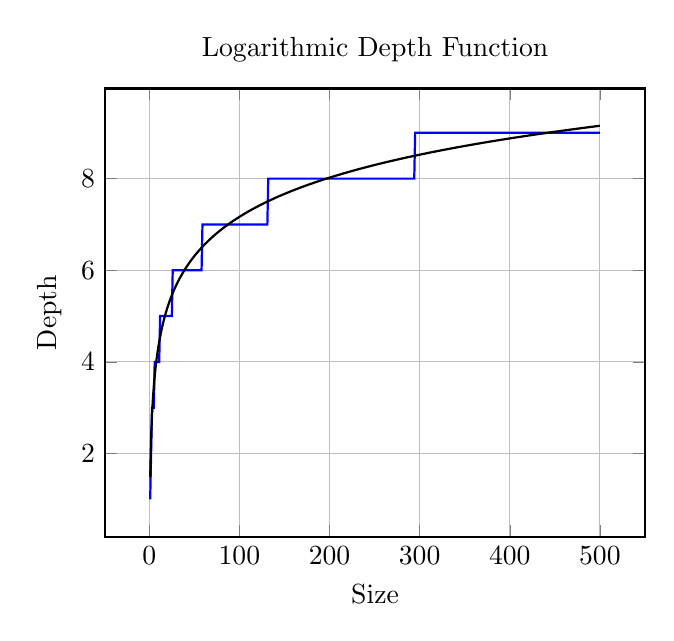
\begin{tikzpicture}
        \begin{axis}[
            xlabel={Size}, 
            ylabel={Depth},
            title={Logarithmic Depth Function},
            domain=1:500, % Adjust range as needed
            samples=500,
            grid=major,
            thick
        ]
            % Define constants
            \pgfmathsetmacro{\M}{1.235}    % Scaling factor
            \pgfmathsetmacro{\L}{0.906}    % Log multiplier
            \pgfmathsetmacro{\C}{-1.6}    % Offset
            \pgfmathsetmacro{\maxD}{10} % Maximum depth
            
            % Plot the function
            \addplot[blue, thick] {min(\maxD, max(0, round(\M * ln(\L * x) - \C)))};
            \addplot[black, thick] {\M * ln(\L * x) - \C};
        \end{axis}
    \end{tikzpicture}
    }%
    \caption{Plot Of Depth Function}
\end{figure}

The formula states that the depth can be set to any logarithmic curve with respect to size, as defined by three variables(M = multiplication, L = logarithmic, C = constant), provided that it satisfies $max\_depth \geq depth \geq 0$. The values of M, L, and C must be set before run-time but can be optimised from testing and applying gradient descent. There are two ways the formula can be used to set the depth:

\begin{itemize}
    \item Beginning: Set the optimal depth at the start for the whole length of the algorithm
    \item Iteratively: Set the optimal depth each iteration of DLACIH
\end{itemize}

Setting it at the beginning means DLACIH will behave like SLACIH, but it guarantees that it will produce a sufficiently good result. Setting it in each iteration alters the design of DLACIH from SLACIH, enabling finer tuning and further research into optimal curves. As the algorithm progresses(high sparsity), more nodes are added to the route, and the proximity of clusters to multiple route nodes increases(low sparsity). Thus, a lower look-ahead depth is more effective towards the end, whereas a higher look-ahead depth is more beneficial at the beginning.

\begin{figure}[H]
    \centering
    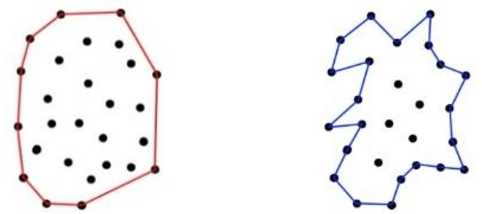
\includegraphics[width=0.8\textwidth]{sections/image/Classification-of-convex-and-concave-hull-Adapted-from-6.png}
    \caption{High(Left) vs Low(Right) Sparsity}
    \cite{sparity-picture}
\end{figure}

\subsubsection{Adaptive Dynamic}
Instead of applying statistics(Section\ref{SDynamic}), a logical step can be added to aid in the dynamic look-ahead process\cite{Strimel2023}. This typically involves an evaluation of the previous iteration(s) \cite{mamou2024dynamicspeculationlookaheadaccelerates} or information gathering\cite {Strimel2023}. 

When evaluating previous iterations, an approach similar to the Lin-Kernighan adaptive selection\cite{Lin1973} can be used(Figure\ref{sporatic}). Changing the depth of look-ahead is beneficial in avoiding local minima that are present within a certain range of depths. By adjusting the depth(Equation\ref{osilatingdepth}), the heuristic can proceed with more promising additions that would have been hindered by pitfalls otherwise.

\begin{equation}
    depth = \min(max\_depth,\  \max(0,\ M\cdot\ln(L\cdot size)\ - C + \tcboxmath[boxmath={red}{displacement}]{D}\cdot\sin(\tcboxmath[boxmath={blue}{sparitrty}]{F\cdot\#iteration}))))
    \label{osilatingdepth}
\end{equation}

\vspace{-0.5cm}

\begin{tikzpicture}[remember picture, overlay, font=\sffamily]
\draw[red,->] (displacement.north) --++(120:5mm) node[anchor=south]{Amplitude};
\draw[blue,->] (sparitrty.north) --++(90:5mm) node[anchor=south]{Frequency};
\end{tikzpicture}

\begin{figure}[]
    \centering
    \resizebox{0.7\textwidth}{!}{%
    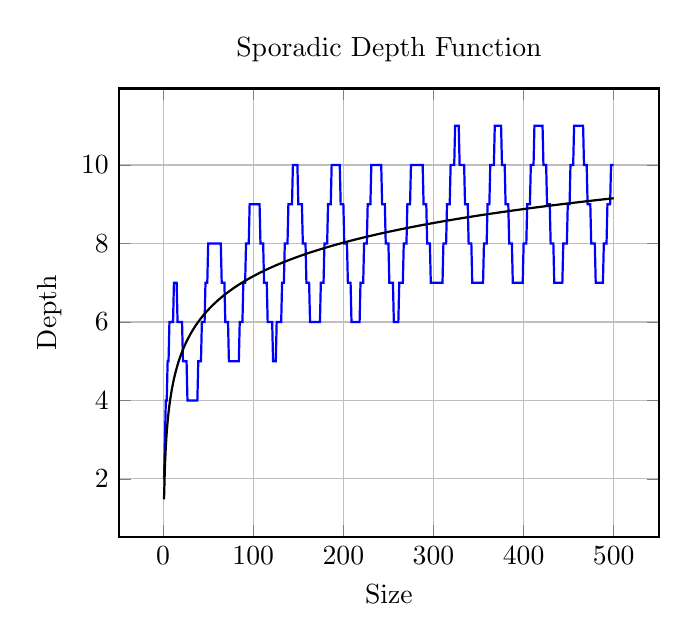
\begin{tikzpicture}
        \begin{axis}[
            xlabel={Size}, 
            ylabel={Depth},
            title={Sporadic Depth Function},
            domain=1:500, % Adjust range as needed
            samples=500,
            grid=major,
            thick
        ]
            % Define constants
            \pgfmathsetmacro{\M}{1.235}    % Scaling factor
            \pgfmathsetmacro{\L}{0.906}    % Log multiplier
            \pgfmathsetmacro{\C}{-1.6}    % Offset
            \pgfmathsetmacro{\maxD}{100} % Maximum depth
            
            % Plot the function
            \addplot[blue, thick] {min(\maxD, max(0, round(\M * ln(\L * x) - \C + 2*sin(8*x))))};
            \addplot[black, thick] {\M * ln(\L * x) - \C};
        \end{axis}
    \end{tikzpicture}
    }%
\caption{Plot Of Sporadic Depth Function}
\label{sporatic}
\end{figure}

If acting upon information gathered from the current state, logical assumptions can be used to define the depth. Adding a step that adaptively changes the depth based on the proximity to other nodes can help avoid poor representation in the cost function. A crude method for defining closeness is to count the number of nodes within a specified distance of the node. The closeness cut-off can be defined based on an arbitrary size(Figure\ref {closesearch}), statistical assumptions of the problem(such as the mean value), or the best efforts of previous iterations.

\begin{figure}[H]
    \centering
    \includegraphics[page=13, width=0.8\textwidth]{sections/image/dissertationdemo.drawio.pdf}
    \caption{Closeness Search}
    \label{closesearch}
\end{figure}
